\pagebreak

\chapter{Running the Compiler}
\label{chap:run3pl}


    The 3PL compiler is written in Java. It can be run on any computing
    platform that supports Java 1.6 or later. The 3PL compiler was developed
    and used in UNIX and MACOS environments, but can be run in a Windows
    environment as well.
    
    To use 3PL only the following are needed -
    \blist
    \item   the jar file - classes/3PL.jar
    \item   the 3PL libraries in sources/include
    \blend
    
    
    A script for running 3PL should be of the form -

    \verb'exec java -Xmx800M -jar .../3PL/classes/3pl.jar -I.../3PL/sources/include  $*'

    The first option of the Java call provides more heap space than default.
    The -I gives the location of the libraries.

    The compiler generates a Xilinx EDIF netlist file, some associated ISE or
    Vivado constraint files and three optional report files. It can then
    optionally run ISE or Vivado to produce a configuration file that can be
    executed on the FPGA (see below).
    

    \section{Environment variables}

        The environment variable {\bf THREEPL\_INCLUDE\_DIRS} gives an
        additional location of 3PL libraries. It is searched following the
        current directory and the directory specified by the command line -I
        option.

        3PL will by default attempt to post-process the configuration by
        executing the procedure postprocess() in xiline/postprocess.3pl,
        which runs the Xilinx ISE or Vivado tools. The post-processing module
        is described in \autorefph{ch:pp}.
        
        If manual invokation of place-and-route tools is prefered
        then the post-processing can be supressed by
        giving the -s option or by including the following in the 3PL
        source -
        \begin{lstlisting}[gobble=12, language=threepl]
            directive("skipPostProc", true)
        \end{lstlisting}
        
        If 3PL post-processing is to be used then the environment variable
        {\bf XILINX} must be set to the installation directory of the Xilinx
        post-processing tools, typically {\bf /opt/Xilinx} or similar. This
        directory would have been selected when the Xilinx tools (either ISE
        or Vivado) were installed. The standard Xilinx installation structure
        under this directory is assumed. It can be overridden by a 3PL
        directive of the same name.

        The following environment variables should not normally be defined by
        the user, but may be required in unusual situations -

        {\bf XILINX\_ISE}. Specifies a precise version of Xilinx ISE to use,
        for example  {\bf /opt/Xilinx/14.7i}. It can be overridden by a 3PL
        directive of the same name. This overrides the {\bf XILINX}
        environment variable, if defined. Normally the 3PL post-processing
        code will choose the newest version appropriate for the device.

        {\bf XILINX\_VIVADO}. Specifies a precise version of Xilinx Vivado to
        use, for example  {\bf /opt/Xilinx/Vivado/2019.1}. It can be
        overridden by a 3PL directive of the same name. This overrides the
        {\bf XILINX} environment variable, if defined. Normally the 3PL
        post-processing code will choose the newest version appropriate for
        the device.


    \section{Generating EDIF}
    
        The 3PL compiler is run by -
        \begin{verbatim}
        3pl {-Idirectories} {-dhlpst} name
        \end{verbatim}
        where the source file is "name.3pl" (the file name extension need not
        be given in the call to the compiler, though it is accepted). The
        file name argument may be a path containing "/"s.
        There must be only one source file argument.

	The {\em design name} is derived from the source file name argument by
	removing the trailing ".3pl" if present and removing the preceding
	file path up to the rightmost "/" if any.

	The design name may be set by a command line option {\bf -N name}.
	It may also be changed by calling inbuilt procedure
        {\bf designname()} where the string argument supplies a new design name.
        The command line option overrides the inbuilt procedure call which in
        turn prevails over the default derivation from the file name.
        
        The design name is also changed if inbuilt procedure {\bf export()} is
        called to create a logic core EDIF file.
	\index{constraint}
        
	The design name should comprise only alphanumeric characters or "\_"
	(underscore). Any other characters are silently converted to "\_".
	This is to ensure the design name matches the output file names and
	also observes EDIF identifier name restrictions. 

	The compiler will create a Xilinx EDIF netlist file called "name.edn"
	and either a Xilinx ISE constraint file, "name.ncf", or a Vivado
	constraint file, "name.xdc", where "name" is the design name.
        
        The {\bf -I} option specifies a ":"-separated list of directories
	to be searched for files to be included by {\bf source} and
	{\bf module} statements. There may be more than one {\bf -I} and they
	may precede or follow the source file name.
        The "-I" may be separated from its list by spaces, i.e. the list is
        the following argument. Directories are searched in the order -
        current directory, {\bf -I} option lists in order, then finally the
	3PL library directory.
	Therefore, source/module files may be preempted by including alternative
	versions earlier in the directory search path.
        
        To write the three output files to a directory other than the current
        directory a {\bf -o} option can be used. The directory name can
        be appended to the {\bf -o} or can be the following argument. The
        directory will be created if it does not exist.
        
        The call options are - \label{options}
        \blist
        \item   -c - compile only, do not execute
        \item   -d - display the interactive netlist schematic window after
                outputing an EDIF netlist
        \item   -D d=s - define a directive d whose value is string s
        \item   -f - force compilation even if sources have not been changed
        \item   -F - error messages use full path names rather than file names
        \item   -G - use gates rather than LUTs to help optimisation
        \item   -h - print a help message
        \item   -i - intermediate code only
        \item   -I d1:d2:.. - list of directories to search for libraries
        \item   -l - annotate printed TDE list with source file locations
        \item   -n - print a list of netlist net identifiers and their
                equivalent signal names to a file 'name'.net
        \item   -N name - change design name to 'name'
        \item   -o dir - write file to directory 'dir'
        \item   -p - print the TDE list prior to optimisation
        \item   -R - just print token generator output - testing only
        \item   -r - generate a verbose report to file 'name'.rpt
%        \item   -S - run the simulator instead of producing output code
        \item   -s - skip post-processing
        \item   -T - print the TDE list (including signal definitions)
        \item   -t - print the TDE list (excluding signal definitions)
        \item   -V - print the compiler version information 
	    		(with -v, prints more)
        \item   -x - suppress netlist code optimisation - testing only
        \item   -X - development mode - testing only
        \item   -Y - print clock domain resolutions (compiler diagnostic)
        \blend
        
        3PL will by default check the times of last modification of all referenced
        source and library files and the compiler make date. If all of these are older
        than the output netlist file and report file the compiler will exit without
        compiling and executing. This can be overridden by using the -f option to
        force compilation and execution.
        
        At the end of netlist generation 3PL will execute any post-processing
        modules. If this is not desired the -s option will cause this to
        be skipped.
        
        The -r option causes a detailed report to be produced in file {\em
        design\_name}.rpt.
        
        The -t option will result in a listing of the intermediate code in file
        {\em design\_name}.icl. The -l, -p and -T options modify the
        intermediate code listing and are only used for compiler testing.
        
        The -c option terminates 3PL after parsing the source file.
        
        The -i option terminates 3PL after immediate execution.
        
        The -R, -x, -X and -Y options are only used for compiler testing.
        
        The -D option defines a directive. The directive may be just a
        key, in which case a directive of type "log" with that key and value
        {\bf true} will be created. If key=value is given then the directive
        will be given the specified value and its type will be as appropriate
        for the value ("log", "int" or "float"). Space between the -D and the
        key is optional.
        
        The -G option replaces many LUTs normally produced by the code generated
        with nested gates. The logic remains the same but the use of nested
        gates instead of explicit LUTs may change the way the vendor
        place-and-route software optimises and packs the logic which in turn may
        change the ease, or lack thereof, with which the timing contraints can
        be met. Thus when timing constraints fail to be met trying the -G option
        may improve the situation. The same effect can be achieved by setting
        directive {\bf gatesNotLUTs} true prior to completion of immediate
        execution.

        -I, -o, -D and -N may each be, but need not be, separated from its
        argument by spaces.
        
        These options also set associated directives and for most of them
        the directives can also be set during immediate execution - see
        \autorefph{sec:directives}.
        
        If 3PL is called with no command line arguments, it pops up a GUI to
        open the file.
        
        \scalebox{0.5}{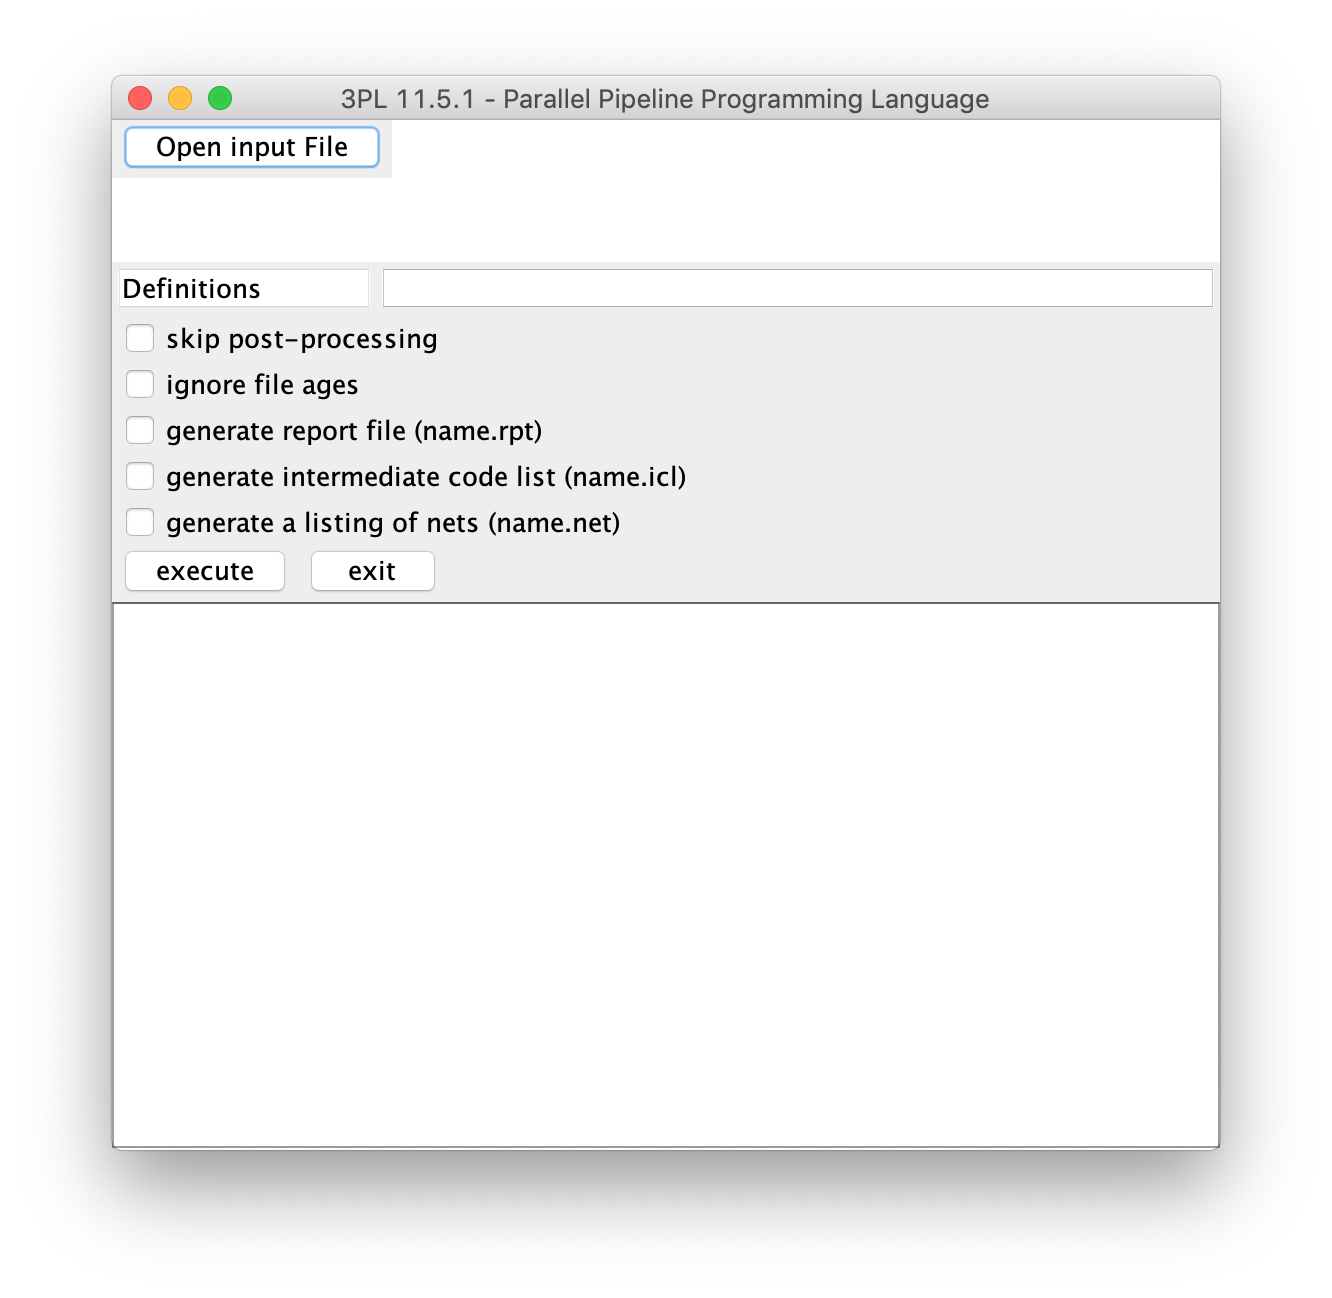
\includegraphics{3PL_GUI}}
        
        The GUI has text fields to specify the source file and any directives to
        define, buttons to set some options and a button to start (parsing,
        immediate execution and then code generation). The output appears in a
        scrollable text window. A file can be repeatedly compiled and executed
        by a single button press. Run this way it is still convenient to run via
        a script so that the library directory is specified and the Java memory
        heap maximum size is set. Directive definitions are space-separated and
        may be {\em name}=value or simply {\em name}. The value may be an
        integer, floating point or the strings "true" or "false". If none of
        those then it will be assumed to be a string value, any enclosing double
        quotes being removed. Where just a directive name is given it will be
        type "log" (boolean) with value TRUE. If the directives string is
        erroneous it will change colour to red.


        Unfortunately the 3PL compiler terminates immediately on most parsing
        errors. This means that you can only fix one error at a time. Making
        the compiler continue following a parsing error is something the author
        has not yet worked out how to accomplish with the compiler compiler
        that was used.

        The error messages have been designed to be as clear and informative as
        possible. However, the following parse error is an exception -
        \begin{verbatim}
        Parse error: file 'prog.3pl' line 2
        Encountered "#m#prog.3pl#2#\n in column 1.
        Was expecting one of:
            "break" ...
            "calling." ...
            "case" ...
            .
            .
            .
        \end{verbatim}
        This has resulted from unmatched braces around a module definition
        in a file included via a {\bf module} or {\bf source} statement!

        An immediate execution error causes termination, which is reasonable.
        
        If a post-processing module is provided then conditional code within
        it will carry out place-and-route and any other such tasks. This is
        described in the next section.
        

    \section{Generating Xilinx FPGA and CPLD configurations}\label{sec:xpp}
    
        See also \autorefph{ch:pp}

    	3PL post-processing code will by default run the Xilinx ISE or Vivado
	tools to transform the EDIF and constraint files generated by 3PL into
	configuration files that may be downloaded into the device for execution.
	To prevent this either the -s option or the "skipPostProc" directive must
        be set true. This might be done where 3PL is executed on a different
        host to that of the place-and-route tools or where the user prefers
        to run the place-and-route separately for some reason.

	The post-processing code automatically selects the Xilinx tool set and
	version based on the FPGA or CPLD part. Xilinx Vivado is used for 7-series
	FPGAs, and ISE for all other FPGAs and CPLDs.

	The code uses the newest installed version of ISE or Vivado, found under
	the installation directory specified by the {\bf XILINX} environment
	variable or 3PL directive, that supports the part.
	This is because Xilinx dropped support for older parts as newer
	versions of ISE were released, and older versions of the software did
	not support later parts.

	This version can be overridden if necessary using either the
	{\bf XILINX\_ISE} environment variable or 3PL directive, or the
	{\bf XILINX\_VIVADO} environment variable or 3PL directive, as
	appropriate. The need to do so should be rare.

	Actual post-processing uses a 'recipe' file. For ISE the recipe file is
	a simple list of ISE commands to run. The default recipe for FPGAs is 
	the file {\bf xilinx/ise\_fpga.cmd} -

        \begin{verbatim}
	ngdbuild @designName@
	map -detail -w -timing -ol high -pr b @designName@
	par -w -ol high @designName@ @designName@.ncd
	bitgen -m -w -g LCK_cycle:4 -g GTS_cycle:1 @designName@
        \end{verbatim}

	Items in the recipe file enclosed with \verb+@+ characters are replaced
	with the 3PL directive of the same name. Generally only the "designName"
	and "part" directives are useful.
	The ISE commands are executed in order, until one of them returns an
	error status or the script is completed.

%        where {\em xtimerr} is the script
%        \begin{verbatim}
%        \#! /usr/bin/sh -f
%        ggrep -q 'All constraints were met' $1.par
%        if ($status == 0) then
%            /bin/rm -f $1.twr $1.err
%        else
%            trce -e 50 -skew $1
%        endif
%        \end{verbatim}
%        \index{constraint!timing}
%        \index{timing constraint}
%        This conditional executes the Xilinx tool {\bf trce} if timing
%        constraints were not met during the place-and-route. This creates
%        a report file "name.twr"

	For Vivado the recipe file is a Tcl script run in the Vivado Tcl
	interpreter in non-project mode.
	The same \verb+@+-substitution is performed on the recipe first.
	The default recipe is {\bf xilinx/vivado.tcl} -

        \begin{verbatim}
	# read the EDIF netlist file into Vivado
	read_edif @designName@.edn

	# read the constraints file into Vivado (if there is one)
	if {[file exists @designName@.xdc]} {
	    read_xdc -ref @designName@ @designName@.xdc
	}

	# place and route the design
	link_design -top @designName@ -part @part@
	opt_design
	power_opt_design
	place_design
	phys_opt_design
	route_design
	phys_opt_design
	write_checkpoint -force @designName@.dcp

	# emit the reports
	report_timing_summary -file @designName@.tim
	report_io -file @designName@.pad
	report_utilization -file @designName@.xlxs
	report_clock_utilization -file @designName@.clku

	# write bitstream
	write_bitstream -force @designName@.bit
	\end{verbatim}

        Note that a checkpoint file is created so that it can be read into
	Vivado in GUI mode and the design layout can be examined.

	Both ISE and Vivado are run in the 3PL compiler output directory, as
	specified by the -o option. This means that the recipe files can expect
	their input netlist and constraint files in the 'current' directory,
	and the many output files from the ISE and Vivado programs are also
	written to the output directory.

	The default ISE and Vivado recipe files should be adequate for most
	3PL programs, but if necessary they can be overridden by defining the
	3PL directive "postProcessRecipe". This should be the filename of the
	recipe, not the recipe itself, and is searched for on the same
	include directory path as the 3PL {\bf source} and {\bf module}
	statements. It would typically be located within the user's source
	code.

	The voluminous output from the ISE and Vivado programs is filtered
	so that only warning and error messages are printed. This may be
	changed using the 3PL directive "postProcessFilter", which should have
	string values "error", "critical", "warning", "info", or "all".
	The 3PL compiler -v option (verbose) has the same effect as "all".
        
	If the 3PL directive "postProcessAppendFile" is defined and the file
	it names is readable, it is appended to the FPGA configuration file
	with a separator string. Board support modules use this to attach a
	text report or information file to the configuration. This can be
	examined to determine the provenance of the configuration.
	The extra data has been found not to upset FPGA configuration loaders,
	and it seems to be ignored. 

	If the 3PL boolean directive "postProcessCompress" is defined and true
	the FPGA configuration file is compressed using gzip.

    \section{The report file}
    
        The report file is produced when the -r option is provided on calling
        3PL. It has the following sections -
        
        {\bf \underline{Source files}}
        
            Source files are listed starting with the primary source file in the
            3PL call and then files inluded by {\bf module} or {\bf source}
            statements the order they are read. The list entries are indented
            to reflect the nesting depth of each included file.
            
            Each line has three components, a label, a directory path and the
            3PL source file in that directory.
            
            The label is "SRC" for a file included by a {\bf source} statement
            and is "FMODn", where 'n' is 1, 2, 3 etc. for a file included by
            a {\bf module} statement.
            
            Signal names are constructed using the file path as a prefix. This
            generates quite long signal identifiers. To reduce this the "FMODn"
            labels are used in place of directories. Thus unique signal names
            are still ensured but are shortened. When reading the intermediate
            code list the path string of a source file can be determined by
            consulting the source file list and matching the label.
        
        {\bf \underline{Leader modules main module and trailer modules}}
        
            Each leader module is listed as it is executed using the identifying
            string supplied in the source code. The ordering number is also
            listed.

            The main module is then executed

            Finally each trailer module is listed as it is executed, again using
            the identifying string supplied in the source code. Again the
            ordering number is also listed.

            In any of these there may be warnings printed or there may be an
            exception thrown for a code error in the module.
            
        {\bf \underline{Logic for variables}}
        
            The logic for target variables is created. Variables which are
            unused are listed and code for them is not generated. There may
            also be interspersed warnings about possible assignment conflicts.
            These can not usually be resolved by 3PL and it is up to the
            programmer to verify that these assignments are mutually exclusive
            by the logic of the program.
            
        {\bf \underline{Queue variables with multiple sinks}}
        
            Queue variables which have more than one destination (reader)
            are listed as a convenience to the programmer. The rules for
            multiple queue sinks are complicated and this list is a reminder
            to the programmer to verify that modules which pop entries from
            queues are correctly structured. A coding error here can be quite
            difficult to resolve.
            
        {\bf \underline{Clock variables}}
        
            Clock variables, as with all
            variables, are usually passed as inputs or outputs to modules or
            procedures, in each case acquiring a new identifier. These multiple
            identifiers are all equivalent as the named signals are connected.
            3PL attempts to extract the most meaningful of these for each
            distinct clock and use that identifier in all occurrences of the
            clock signal.
            
            These primary identifiers are listed in a section titled "clocks
            driving logic".
            
            Following this all other clocks are listed. These are intermediate
            clocks between input buffers, clock managers and clock buffers and do
            not drive clock inputs of logic elements.
            
        {\bf \underline{Directives}}
        
            This section lists all directives at completion of immediate
            execution.
            
        {\bf \underline{Intermediate code optimisation}}
        
            This section lists a few details such as optimisation stages
            and the number of passes in each. This is probably mainly of
            interest to the 3PL maintainer.
            
            A detailed list of clocks appears again here, in this case showing
            wihch are unused and which are connected to other clock signals
            and are aliases. These latter are often identifiers of clock
            variables which are module or procedure parameters.
            
        {\bf \underline{Generating EDIF code}}
        
            This section reports statistics on netlist optimisation processes
            and passes. It also lists the number of elementary FPGA elements
            of each type generated. Finally CPU and elapsed time for
            parsing, emmediate execution etc. are listed along with memory
            usage.
        
        
        
        
        

    \section{Netlist identifier file}

        When calling 3PL and the {\bf -n} option is given, a list of netlist
        file net identifiers will be written to file {\em design\_name}.net.
        Each identifier is listed at the beginning of a line and is followed
        by a colon and then a list of equivalent net identifiers. If the {\bf
        -o} option is also supplied then the file will appear in the
        specified directory. The list of equivalent net identifers can be
        used to identify source program variable identifiers associated with
        signal identifiers appearing in the netlist file or in any vendor
        place-and-route report files.
        
    \section{The intermediate code list file}
    
        The intermediate code produced by the 3PL compiler following immediate
        execution can be listed in file {\em design\_name}.icl by using option -t
        when calling 3PL. If option -pt is given instead the intermediate code
        prior to optimisation will also be listed. The listing will not include
        signal declarations (SIG elements - see below) but these can be included
        by using -T and -pT.
        
        The intermediate code is described in \autorefph{intermediatecode}.
        
        Examination of the intermediate code can be very useful in verifying
        what 3PL has generated and in attempting to determine signal paths which
        do not meet timing constraints. The listing has been formatted to be
        concise but human-readable.
            
    \section{Netlist display and debugging}
    
        The compiler can also display the generated netlist as a schematic
        if the {\bf -d} option is given. In this window elements and nets of the
        EDIF netlist can be traced. This feature is not very useful and
        indeed has not been used for years. In the interim it appears to
        have atrophied. It will be fixed when time permits. A version
        displaying the intermediate code list would be much more useful.
        
        The display window has a text area on the bottom right in which to
        click and enter a signal, pin or block identifier. The type of
        identifier is selected by clicking on buttons "signal", "pin" or
        "block".
        
        For signals a signal identifier, or part of an identifier, is entered
        followed by a return. If the string entered is an identifier and it is not
        a substring of any other identifier the element which is the source of the
        signal will be displayed in the window. If the string entered is a
        substring of multiple identifiers then a sorted list of those identifiers
        will appear in a scrollable pop-up list. Left-clocking an identifier in the
        list will display its source element and hide the list. If the string is
        also a complete identifier as well as a substring of other identifiers then
        that identifier will appear at the head of the list. Note that the signal
        identifiers are those present in the netlist file and these will often have
        been translated from the intermediate code identifiers by replacing
        dots and brackets by underscores (these characters are not accepted in
        netlist identifiers).
        
        For pins the FPGA pad designator must be entered. The block attached to
        the pin will be displayed.
        
        For blocks the unique block identifier must be provided.
        
        An element in the schematic window may have any input wire
        left-clicked to display its source element(s) or any output wire
        left-clicked to display its destination element(s). A left click in
        the body of an element will expand all its inputs (GND and VCC
        inputs are not expanded). A middle click on an input will remove the
        displayed source element for that input and a middle click in an
        element will remove all displayed input source elements. If an
        element is right-clicked its properties will be displayed in a
        pop-up text window. These properties include RAM and flip-flop
        initialisation, LUT initialisation and associated equation and any
        UCF or NCF file strings.
        
        {\bf Note: the schematic display software was written to aid
        compiler development and debugging. The display sometimes
        malfunctions as it has not been completely debugged. Because
        the display tool is probably of little if any use to normal
        3PL users its debugging has a low priority.}
